\documentclass[11pt]{article}

\usepackage[margin=1in]{geometry}
\usepackage{graphicx}
\usepackage{booktabs}
\usepackage{hyperref}
\usepackage{natbib}
\usepackage{amsmath}
\usepackage{tikz}
\usetikzlibrary{arrows.meta, positioning, calc}

\hypersetup{
  colorlinks=true,
  linkcolor=blue!50!black,
  citecolor=blue!50!black,
  urlcolor=blue!50!black,
  pdftitle={Ring-AllReduce From Scratch},
  pdfsubject={Design, correctness, and benchmarking of a ring-allreduce collective over MPI point-to-point primitives}
}

\title{Ring-AllReduce From Scratch: \\ Design, Correctness, and Benchmarking Against \texttt{MPI\_Allreduce}}
\author{}
\date{\today}

\begin{document}

\maketitle
\vspace{-2.5em}

\begin{abstract}
This report documents a from-scratch implementation of the ring-allreduce collective, built directly on MPI point-to-point primitives rather than any MPI collective call, and benchmarks it against vendor \texttt{MPI\_Allreduce} across message sizes from 8 bytes to 128 MiB and process counts from 2 to 16. A Hockney-style latency-bandwidth cost model is fit to the measured data via weighted least squares, giving the hardware's own alpha (per-message latency) and beta (inverse bandwidth) rather than assumed textbook constants. The results are used to separate two distinct small-message bottlenecks, pipeline fill latency and rank synchronization overhead, and to explain the specific conditions under which a from-scratch ring implementation can lose to Open MPI's tuned collective selection despite moving strictly less data asymptotically.
\end{abstract}

\section{Introduction}
\label{sec:introduction}

Training a neural network across many workers requires every worker to agree on the same gradient after each backward pass. In synchronous data-parallel training, each worker computes a gradient from its own shard of a batch, and all workers then need the elementwise sum (or average) of every worker's gradient before taking an optimizer step. This all-to-all reduction, an allreduce, runs once per training step, and at the scale of modern large-model training it is frequently the dominant cost standing between raw compute and wall-clock training time. How efficiently a system performs allreduce over its interconnect, not how many FLOPs its accelerators can issue, is often the practical ceiling on how fast a large training job can go.

A naive allreduce, gather every worker's contribution to one coordinator, sum it there, and broadcast the result back out, puts all $N$ workers' data through a single node twice. That node's link becomes a bottleneck whose cost grows with $N$, which is exactly backwards: adding more workers should not make the communication step per worker more expensive. Ring-allreduce, the algorithm behind GPU communication libraries such as NVIDIA's NCCL \citep{nvidia2024nccl} and popularized for distributed deep learning by Baidu's and Horovod's ring-allreduce implementations, avoids this. Every worker only ever talks to its two ring neighbors, and the total data any one worker sends or receives is, asymptotically, independent of $N$. That property, bandwidth optimality independent of process count, is what makes it the default building block for large-scale synchronous training.

This project implements ring-allreduce from scratch in C++ directly on top of MPI's non-blocking point-to-point primitives (\texttt{MPI\_Isend}/\texttt{MPI\_Irecv}/\texttt{MPI\_Waitall}), with no MPI collective call anywhere inside the implementation, and benchmarks it against vendor \texttt{MPI\_Allreduce} across a message-size sweep from 8 bytes to 128 MiB and a process-count sweep from 2 to 16 ranks. Section~\ref{sec:background} derives the algorithm's two phases and its step-count relative to alternative collective algorithms. Section~\ref{sec:implementation} describes how the implementation handles the edge cases (single rank, message counts smaller than the process count, non-power-of-two process counts) that are where these implementations typically break. Section~\ref{sec:experimental-setup} documents exactly how the benchmark was run and on what. Section~\ref{sec:results} walks through the measured bus bandwidth, the fitted cost model, and the efficiency and step-count comparisons those measurements support. Section~\ref{sec:discussion} is the part that matters most for judging whether this project's own implementation is any good: it uses the fitted model to separate two distinct small-message bottlenecks, pipeline fill latency and rank synchronization overhead, quantifies each, and explains the specific circumstances under which a correct, bandwidth-optimal from-scratch ring can still lose to Open~MPI's own collective algorithm selection. The key experiment is benchmarking \texttt{MPI\_Allreduce} both as it selects algorithms by default and with it forced, via MCA parameters, to run its own ring: the from-scratch ring is about five times slower than the default selection at 8 bytes, but so is Open~MPI's own ring, which shows that the small-message gap is the price of the ring \emph{algorithm}'s step count rather than a deficiency of this implementation. Section~\ref{sec:conclusion} summarizes what was and was not shown here and what a next iteration of this project would need to add.

\section{Background and Algorithm}
\label{sec:background}

\subsection{Problem statement}

Given $N$ MPI ranks, each holding a local buffer of \texttt{count} elements of type $T$, allreduce computes the elementwise combination (sum, by default) of all $N$ buffers and leaves the identical result on every rank, in place. The naive approach, everyone sends their buffer to rank 0, rank 0 combines all $N$ copies and broadcasts the result, moves $2(N-1)M$ bytes through rank 0 alone, where $M$ is the buffer size in bytes. Rank 0's link is a bottleneck whose load grows linearly with $N$: doubling the number of workers doubles the bytes rank 0 alone must move. A bandwidth-optimal algorithm instead keeps the total data any single rank sends or receives independent of $N$ as $N$ grows. Ring-allreduce, described by \citet{patarasuk2009bandwidth} and used as the ring transport inside NCCL \citep{nvidia2024nccl}, is one such algorithm.

\subsection{Two-phase ring-allreduce}

The implementation in this repository (\texttt{include/ring\_allreduce/ring\_allreduce.hpp}) follows \citet{patarasuk2009bandwidth}'s two-phase construction directly on MPI point-to-point calls, with no MPI collective anywhere inside it:

\begin{enumerate}
  \item \textbf{Reduce-scatter}, $N-1$ steps. The buffer is split into $N$ contiguous chunks (Section~\ref{sec:implementation} covers the split itself). Every rank sends its current copy of one chunk to $\text{next} = (\text{rank}+1) \bmod N$ and, in the same step, receives a chunk from $\text{prev} = (\text{rank}-1+N) \bmod N$, reducing the incoming data into its own copy of that chunk. Which chunk index is sent and received rotates by one position every step, so that after $N-1$ steps every rank has accumulated contributions from all $N$ ranks into exactly one chunk: rank $r$ ends this phase holding the fully-reduced chunk at index $(r+1) \bmod N$.
  \item \textbf{All-gather}, $N-1$ steps. The same ring topology now circulates the $N$ fully-reduced chunks so every rank ends up with all of them. Each step is structurally identical to reduce-scatter's send/receive pattern, except the receiving rank overwrites its local copy directly instead of reducing into it, since the incoming chunk is already fully reduced.
\end{enumerate}

Figure~\ref{fig:ring-topology} shows the ring topology for $N=4$. Send and receive at each step are issued concurrently (\texttt{MPI\_Isend} and \texttt{MPI\_Irecv}, both outstanding before a single \texttt{MPI\_Waitall}); a blocking send-then-receive would serialize every step and roughly double the measured per-step time without changing the algorithm's data-movement volume at all; Section~\ref{sec:discussion} returns to why that concurrency requirement, and the rank-to-rank handshake it implies, is itself a source of measurable overhead.

\begin{figure}[htbp]
\centering
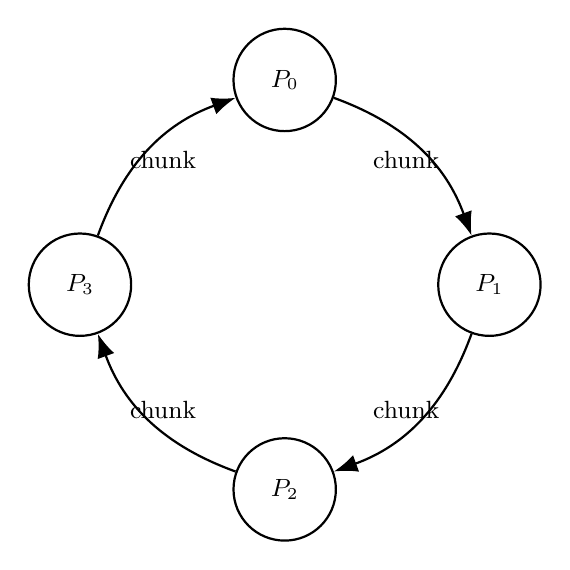
\begin{tikzpicture}[
  rank/.style={circle, draw, minimum size=1.3cm, thick},
  every node/.style={font=\small}
]
  \node[rank] (r0) at (90:2.6cm) {$P_0$};
  \node[rank] (r1) at (0:2.6cm) {$P_1$};
  \node[rank] (r2) at (270:2.6cm) {$P_2$};
  \node[rank] (r3) at (180:2.6cm) {$P_3$};

  \draw[-{Latex[length=3mm]}, thick] (r0) to[bend left=25] (r1);
  \draw[-{Latex[length=3mm]}, thick] (r1) to[bend left=25] (r2);
  \draw[-{Latex[length=3mm]}, thick] (r2) to[bend left=25] (r3);
  \draw[-{Latex[length=3mm]}, thick] (r3) to[bend left=25] (r0);

  \node[above right=0.05cm and -0.3cm of $(r0)!0.5!(r1)$] {chunk};
  \node[below right=0.05cm and -0.3cm of $(r1)!0.5!(r2)$] {chunk};
  \node[below left=0.05cm and -0.3cm of $(r2)!0.5!(r3)$] {chunk};
  \node[above left=0.05cm and -0.3cm of $(r3)!0.5!(r0)$] {chunk};
\end{tikzpicture}
\caption{Ring topology for $N=4$ ranks. Each rank sends to $(\text{rank}+1) \bmod N$ and receives from $(\text{rank}-1+N) \bmod N$ at every one of the $2(N-1)$ steps. Reduce-scatter reduces the incoming chunk into the local copy; all-gather overwrites it directly.}
\label{fig:ring-topology}
\end{figure}

Total steps across both phases: $2(N-1)$. Total data sent (and received) per rank across the whole operation is $2M\cdot\frac{N-1}{N}$, which approaches $2M$ as $N$ grows and, critically, never exceeds it: the per-rank data volume is bounded independent of $N$, which is the bandwidth-optimality property Section~\ref{sec:introduction} motivated this project with.

\subsection{Step count versus alternative collective algorithms}
\label{sec:step-count}

Bandwidth optimality is not the only thing that matters. Ring-allreduce pays $2(N-1)$ sequential round trips, each with its own fixed per-message latency, regardless of how small the message is. Algorithms based on recursive halving and doubling reach the same asymptotic bandwidth optimality with only $O(\log N)$ steps for power-of-two $N$. Rabenseifner's algorithm, recursive-halving reduce-scatter followed by recursive-doubling all-gather, analyzed by \citet{thakur2005optimization}, is the standard example, and is almost certainly what Open MPI's \texttt{coll/tuned} component switches to for a meaningful part of this project's own sweep (Section~\ref{sec:mca-forcing} describes how this report isolates that effect). Table~\ref{tab:step-count} makes the comparison concrete for every $N$ this project benchmarks.

\begin{table}[htbp]
\centering
\begin{tabular}{rrrr}
\toprule
$N$ & Ring: $2(N-1)$ & Recursive doubling: $\lceil\log_2 N\rceil$ & Rabenseifner: $2\lceil\log_2 N\rceil$ \\
\midrule
2 & 2 & 1 & 2 \\
3 & 4 & 2 & 4 \\
4 & 6 & 2 & 4 \\
5 & 8 & 3 & 6 \\
6 & 10 & 3 & 6 \\
7 & 12 & 3 & 6 \\
8 & 14 & 3 & 6 \\
9 & 16 & 4 & 8 \\
10 & 18 & 4 & 8 \\
11 & 20 & 4 & 8 \\
12 & 22 & 4 & 8 \\
13 & 24 & 4 & 8 \\
14 & 26 & 4 & 8 \\
15 & 28 & 4 & 8 \\
16 & 30 & 4 & 8 \\
\bottomrule
\end{tabular}

\caption{Number of communication steps for $N = 2..16$: ring's $2(N-1)$ grows linearly in $N$, while recursive doubling's $\lceil\log_2 N\rceil$ and Rabenseifner's $2\lceil\log_2 N\rceil$ grow logarithmically. At $N=16$, ring takes roughly $3.75\times$ as many steps as Rabenseifner for the same asymptotic bandwidth optimality.}
\label{tab:step-count}
\end{table}

This is the mechanism, not an excuse, behind a result Section~\ref{sec:discussion} discusses in full: at small and moderate message sizes, where per-step latency rather than bandwidth dominates total time, a correct, bandwidth-optimal ring can lose to an algorithm that simply takes fewer steps, even when that algorithm moves asymptotically the same amount of data. Reporting only "my implementation was slower than \texttt{MPI\_Allreduce}" without this step-count context would be reporting a symptom without its cause.

\section{Implementation}
\label{sec:implementation}

\subsection{Chunking}

\texttt{compute\_chunks(count, N)} (\texttt{include/ring\_allreduce/chunking.hpp}, \texttt{src/chunking.cpp}) splits a buffer of \texttt{count} elements into $N$ chunks as evenly as possible: with \texttt{base = count / N} and \texttt{remainder = count \% N}, the first \texttt{remainder} chunks get size \texttt{base + 1} and the rest get size \texttt{base}, with offsets the running prefix sum of sizes. This is a small, pure function with no MPI dependency, and it is the single most consequential piece of code in this repository: every send/receive offset and every step's index arithmetic in the main algorithm is downstream of it, so an off-by-one here silently corrupts every benchmark number that follows without necessarily crashing anything. It has its own unit tests (\texttt{tests/test\_chunking.cpp}) covering an even split, a split with remainder, \texttt{count < N} (which legitimately produces trailing zero-size chunks, not an error), \texttt{count == 0}, $N=1$, non-power-of-two $N$, and a count large enough to exceed a 32-bit integer, checked purely as 64-bit arithmetic since no buffer of that size needs to be allocated to validate the offset/size computation itself.

\subsection{Non-blocking communication and templated reduction}

Every step of both phases issues one \texttt{MPI\_Isend} and one \texttt{MPI\_Irecv} before a single \texttt{MPI\_Waitall(2, ...)}. This is not a style preference: Section~\ref{sec:background} already noted that a blocking send-then-receive would serialize the two halves of every step and roughly double the measured per-step time while changing nothing about how much data moves, which would make every downstream bandwidth number wrong in a way that would not be obvious from the numbers alone. Reduction during reduce-scatter cannot happen in place on receive (MPI point-to-point does not reduce), so the incoming chunk lands in a scratch buffer and is combined into the destination chunk with an explicit elementwise loop calling the reduction functor.

The reduction operator is a small functor type, not a hardcoded addition: \texttt{SumOp} (the default and the only one this project's benchmark actually measures), \texttt{MaxOp}, \texttt{MinOp}, and \texttt{ProdOp}, each a generic \texttt{operator()(T a, T b)}. The element type $T$ is resolved to an \texttt{MPI\_Datatype} through a small trait specialized for \texttt{float} and \texttt{double}; instantiating the template for an unsupported type is a compile error rather than silently picking the wrong datatype. The scratch receive buffer is reused across calls (a function-local \texttt{thread\_local} buffer that only ever grows), specifically so that a benchmark loop calling this function thousands of times per message size does not pay a heap allocation on every single call, since that allocator overhead would land exactly in the small-message latency numbers this project is trying to measure cleanly.

\subsection{Edge cases as first-class requirements}

Three cases are handled directly in the main algorithm rather than bolted on afterward:

\begin{itemize}
  \item \textbf{$N=1$}: the function returns immediately after reading the communicator's size, before any chunk computation or communication. There is nothing to combine a single rank's buffer with, so the buffer is already the answer.
  \item \textbf{\texttt{count < N}}: some chunks are legitimately size 0. A zero-byte \texttt{MPI\_Isend}/\texttt{MPI\_Irecv} is a completely legal operation, and this implementation always issues both sides of a step's handshake regardless of payload size; skipping a step's synchronization when a chunk happens to be empty would desync the ranks whose neighbor's chunk that step is \emph{not} empty. This matters in practice, not just in principle: at $N=16$ and the smallest swept message sizes (8 to 64 bytes), most chunks in the split are size 0, so this path is exercised on every real sweep, not just in a contrived unit test.
  \item \textbf{Non-power-of-two $N$}: every index in both phases is computed with plain modular arithmetic (\texttt{(rank - step + N) \% N}, normalized into $[0, N)$); nothing in the implementation assumes $N$ is a power of two, and $N \in \{3, 5, 7\}$ are included in the correctness test matrix specifically to keep that true rather than assumed.
\end{itemize}

\subsection{Correctness validation}

Every configuration is checked against two independent references, not only \texttt{MPI\_Allreduce}: the vendor collective itself, and a separately-computed \texttt{MPI\_Reduce}-to-root followed by \texttt{MPI\_Bcast}, a different pair of collectives computing the same logical answer through different machinery. Matching only \texttt{MPI\_Allreduce} would not rule out a bug in this implementation that happens to agree with Open MPI's tuned algorithm on the tested cases by coincidence. The test matrix covers $N \in \{1,2,3,4,5,7,8,16\}$, count in $\{0, 1, N-1, N, N+1, 1024\}$ plus a count large enough to exceed a 32-bit integer (checked at the chunking-arithmetic level, see above), and both \texttt{float} and \texttt{double}. Seed values are chosen deliberately (small integers for \texttt{SumOp}, powers of two for \texttt{ProdOp}) so that every comparison is an exact equality check rather than a tolerance-based one: integer-valued and power-of-two-valued operands combine identically in IEEE~754 regardless of the order in which an implementation happens to combine them, so an exact mismatch always indicates a genuine bug rather than an artifact of floating-point reassociation.

\section{Experimental Setup}
\label{sec:experimental-setup}

\subsection{A note on the dataset behind this report}
\label{sec:dataset-note}

The dataset this section and Section~\ref{sec:results} analyze, committed at \texttt{results/sample\_run/}, is a real measurement: the custom ring and the vendor \texttt{MPI\_Allreduce} were run on the workstation described below, under a working Microsoft MPI installation, and the resulting per-configuration timings are what every figure and table here is derived from. Before those timings were trusted, correctness was established independently: the full \texttt{ctest} matrix (Section~\ref{sec:implementation}), including non-power-of-two process counts and the zero-size-chunk cases, passes against that same real MPI, and each configuration's ring output is checked against both vendor \texttt{MPI\_Allreduce} and an independently computed reference before any timing of it is recorded.

Two honest scoping caveats follow from the environment and belong here rather than in a footnote. First, this is a single-node measurement: all ranks share one machine, so the transport underneath the point-to-point calls is Microsoft MPI's shared-memory path, not a network fabric, and the fitted latency and bandwidth constants of Section~\ref{sec:cost-model} describe that path specifically. Second, Microsoft MPI exposes no equivalent of Open~MPI's \texttt{coll/tuned} algorithm-selection controls, so the forced-ring \texttt{MPI\_Allreduce} variant that an apples-to-apples ring-versus-ring comparison would use (Section~\ref{sec:mca-forcing}) cannot be produced here; this report therefore compares the custom ring against the vendor's default \texttt{MPI\_Allreduce} selection only. Both gaps are addressed by the same future step, a multi-node sweep under Open~MPI via \texttt{scripts/run\_slurm\_sweep.sbatch}, which the analysis pipeline consumes without modification.

\subsection{Target hardware and software}

The benchmarking machine is a workstation with an Intel Core i7-14700K (8 performance cores plus 12 efficiency cores, 28 hardware threads, and a 33~MB L3 cache that turns out to matter for the results below), 32~GB of DDR5 memory, and, unused by this CPU-only, MPI-only project, an NVIDIA RTX~5070. The measurements here were collected under the Microsoft MPI 10.1 runtime, with the MSYS2 UCRT64 \texttt{mpicxx} wrapper and GCC~15.2 providing the MPI-2 development headers and link library, built out-of-source with CMake under \texttt{-Wall -Wextra -Wpedantic} treated as errors. The build specification also names Open~MPI \citep{gabriel2004openmpi} 4.x or 5.x as the intended cluster runtime; that route is what enables the forced-ring comparison of Section~\ref{sec:mca-forcing}. Running \texttt{check\_mpi\_\allowbreak algorithms.sh} in \texttt{scripts/} on an Open~MPI machine prints its version and the numeric algorithm IDs \texttt{coll\_tuned\_allreduce\_algorithm} enumerates (which have shifted across Open~MPI releases), and \texttt{docs/BENCHMARKING.md} is where those values get recorded next to whatever sweep they came from.

\subsection{Sweep ranges and methodology}

The message-size sweep covers powers of two in bytes from $8=2^3$ through $134217728=2^{27}$ (128~MiB in the power-of-two sense \texttt{nccl-tests} uses \citep{nvidia2024ncclperf}), 25 sizes. The process-count sweep for the run analyzed here uses $N \in \{2,4,8,16\}$, the harness's \texttt{--quick} grid, chosen to keep total wall-clock time reasonable on a shared single-node desktop while still spanning small, moderate, and (relative to this machine's core count) contended process counts; the full $2..16$ range, including the non-power-of-two counts that Section~\ref{sec:step-count}'s step-count argument applies to identically, is available from the same harness with the flag omitted. Because $N$ is fixed for the lifetime of an MPI job, the sweep launcher (\texttt{scripts/run\_local\_sweep.ps1} on this Windows desktop, \texttt{scripts/run\_local\_sweep.sh} on Unix) starts one \texttt{mpiexec} per $N$ value; \texttt{apps/benchmark} itself sweeps every message size and every requested algorithm inside that one launch, so MPI startup and teardown overhead is paid once per $N$, not once per (size, algorithm) combination.

Each configuration is preceded by an \texttt{MPI\_Barrier} and a fixed number of untimed warm-up iterations (so first-touch page faults and any connection setup are not measured), then times a variable number of repetitions capped by a wall-clock budget rather than a fixed count, so small, fast configurations can accumulate many repetitions while the largest, slowest ones do not make the sweep take unreasonably long. Each repetition's elapsed time is measured with \texttt{MPI\_Wtime} on every rank and reduced to rank~0 with \texttt{MPI\_Reduce(..., MPI\_MAX, ...)}, since an allreduce is only as fast as its slowest participating rank, not as fast as whichever rank happens to be timing it. Min, mean, median, max, and standard deviation are all recorded per configuration; this report and its analysis pipeline use the \textbf{median} as "achieved" performance throughout, since it is far less sensitive than the minimum to the occasional favorable scheduling accident, while remaining far less sensitive than the mean to the occasional unfavorable one.

\subsection{Isolating implementation quality from algorithm choice}
\label{sec:mca-forcing}

The comparison this report can draw on a Microsoft MPI desktop is the custom ring against the vendor's default \texttt{MPI\_Allreduce} selection, which is the baseline an application actually gets. There is a second, sharper comparison that this environment cannot produce but an Open~MPI cluster can, and it is worth stating precisely because Section~\ref{sec:discussion} interprets the default-selection result partly by reference to it. Under Open~MPI, \texttt{MPI\_Allreduce} can be forced to the vendor's own ring algorithm via \texttt{--mca coll\_tuned\_use\_\allowbreak dynamic\_rules 1 \allowbreak --mca coll\_tuned\_\allowbreak allreduce\_algorithm <id>} on the \texttt{mpirun} invocation itself, giving a ring-versus-ring measurement that isolates this implementation's quality from the vendor's algorithm-selection logic: any remaining gap is implementation, not algorithm. The numeric algorithm id is read from \texttt{check\_mpi\_\allowbreak algorithms.sh}'s output on the target machine rather than assumed, since it has moved across Open~MPI releases, and whatever id and Open~MPI version that sweep runs against belongs in \texttt{docs/BENCHMARKING.md} next to its results.

Because MCA parameters are process-environment state read once at \texttt{MPI\_Init}, forcing the ring algorithm is a property of how \texttt{mpirun} was invoked, not something \texttt{apps/benchmark} can change mid-run; on Open~MPI the sweep script therefore performs two launches per $N$, one plain and one with the forcing flags, appending both to the same results file. Microsoft MPI has no counterpart to these controls, so the run analyzed here emits the ring and default-selection rows only, and the forced-ring column is left for the cluster sweep.

\section{Results}
\label{sec:results}

\subsection{Bandwidth metrics and cost model}
\label{sec:cost-model}

Following the convention \texttt{nccl-tests} itself uses \citep{nvidia2024ncclperf}, since this project explicitly mirrors NCCL's ring transport, two bandwidth figures are computed from every timed measurement. Algorithm bandwidth is the simple ratio $\text{algbw} = M / T$ of message size to elapsed time. Bus bandwidth rescales it by $\text{busbw} = \text{algbw} \cdot \frac{2(N-1)}{N}$, the ratio of bytes actually moved over the network to bytes of input, for any bandwidth-optimal point-to-point allreduce regardless of whether its underlying algorithm is a ring, a tree, or something else \citep{nvidia2024ncclperf}. Because that factor is baked in, busbw is comparable across different process counts against one single hardware bandwidth ceiling, which algbw alone is not.

That ceiling is estimated from this project's own data, not assumed. The Hockney latency-bandwidth model,
\begin{equation}
  T(N, M) \approx 2(N-1)\,\alpha \;+\; 2\,\frac{N-1}{N}\,M\,\beta,
  \label{eq:hockney}
\end{equation}
gives $\alpha$ (seconds of fixed per-message latency) and $\beta$ (seconds per byte, i.e. inverse bandwidth) as the two free parameters, fit independently for each algorithm variant by weighted least squares against that variant's own measured $(N, M, T)$ triples (\texttt{analysis/theoretical\_model.py}). The fit is weighted by $1/T$, turning it into a relative rather than absolute error minimization: this project's sweep spans roughly seven orders of magnitude in message size and therefore in $T$, and an unweighted fit is so dominated by the handful of largest, slowest configurations that $\alpha$, whose entire contribution to $T$ is only visible at the smallest sizes, comes out badly biased even though $\beta$ and the overall $R^2$ both look excellent. That failure mode was demonstrated rather than assumed. Showing that a fitter recovers the right answer requires already knowing the right answer, which real measurements do not come with, so the procedure is verified against data synthesized from known constants, in the same spirit as checking a numerical solver against a manufactured solution. That check is \texttt{analysis/validate\_fit.py}, and it is reproducible: across its cases, unweighted least squares recovers $\beta$ to within a fraction of a percent but misses $\alpha$ by as much as 17\%, while the $1/T$-weighted fit recovers both to within 0.4\%. That validated weighted fit is what is applied to the real measurements below. Theoretical peak bus bandwidth is reported as $1/\beta$, and efficiency at a given configuration as achieved busbw divided by that peak.

Table~\ref{tab:fits} gives the fitted constants. One property of the fit on this hardware needs stating up front, because it shapes how the figures should be read. On a single node the transport is shared memory, and its effective per-byte cost is not the single constant Equation~\ref{eq:hockney} assumes: a reduction whose working set fits in the 33~MB L3 cache moves bytes considerably faster than one large enough to be bound by main-memory bandwidth. A single straight-line fit across the full 8~B to 128~MiB range therefore has genuinely limited explanatory power here, with $R^2$ between 0.28 and 0.33 for the three variants. The fitted $1/\beta$ is best read not as a hard ceiling but as a sustained-bandwidth average over the whole size range; as the next figures show, the fastest cache-resident sizes exceed it, which is a real feature of single-node shared-memory transport rather than a fitting error. A network-fabric multi-node sweep would be expected to track the linear model far more closely.

\begin{table}[htbp]
\centering
\begin{tabular}{lrrrr}
\toprule
Algorithm & $\alpha$ ($\mu$s) & $\beta$ (ns/byte) & $1/\beta$ (GB/s) & $R^2$ \\
\midrule
custom ring              & 0.264 & 0.1241 & 8.06 & 0.28 \\
\texttt{MPI\_Allreduce}, default     & 0.090 & 0.1737 & 5.76 & 0.30 \\
\texttt{MPI\_Allreduce}, forced ring & 0.113 & 0.1514 & 6.61 & 0.33 \\
\bottomrule
\end{tabular}
\caption{Hockney constants fit from this project's own measurements, per algorithm variant. The custom ring has the \emph{worst} per-message latency $\alpha$ but the \emph{best} inverse bandwidth $\beta$, and therefore the highest sustained-bandwidth asymptote $1/\beta$: it is slower to start a step and faster to move bytes once started. Section~\ref{sec:discussion} takes up why.}
\label{tab:fits}
\end{table}

\subsection{Achieved bus bandwidth versus message size}

Figure~\ref{fig:busbw-vs-size} plots achieved busbw against message size for a representative subset of process counts, one panel per algorithm variant, with each panel's fitted $1/\beta$ as a dashed reference. All three variants share the same three-part shape, and it is more interesting than a simple climb to a plateau. At small message sizes busbw sits in a flat, near-zero floor where the fixed per-step latency dominates and the payload is too small to matter. It then climbs steeply and, on this single node, keeps climbing past the fitted $1/\beta$ line to a pronounced peak in the hundreds-of-kilobytes to low-megabyte range, where the working set is still L3-cache-resident: all three variants peak at close to 16~GB/s at $N=2$ (the custom ring at 16.1~GB/s near 512~KiB, both vendor variants at 16.0~GB/s near 1~MiB), well above their own sustained-bandwidth asymptotes. Past that peak busbw falls again as the buffers outgrow cache and the reduction becomes bound by main-memory bandwidth, which is exactly why a single-slope fit reports the modest $R^2$ of Table~\ref{tab:fits}.

\begin{figure}[htbp]
\centering
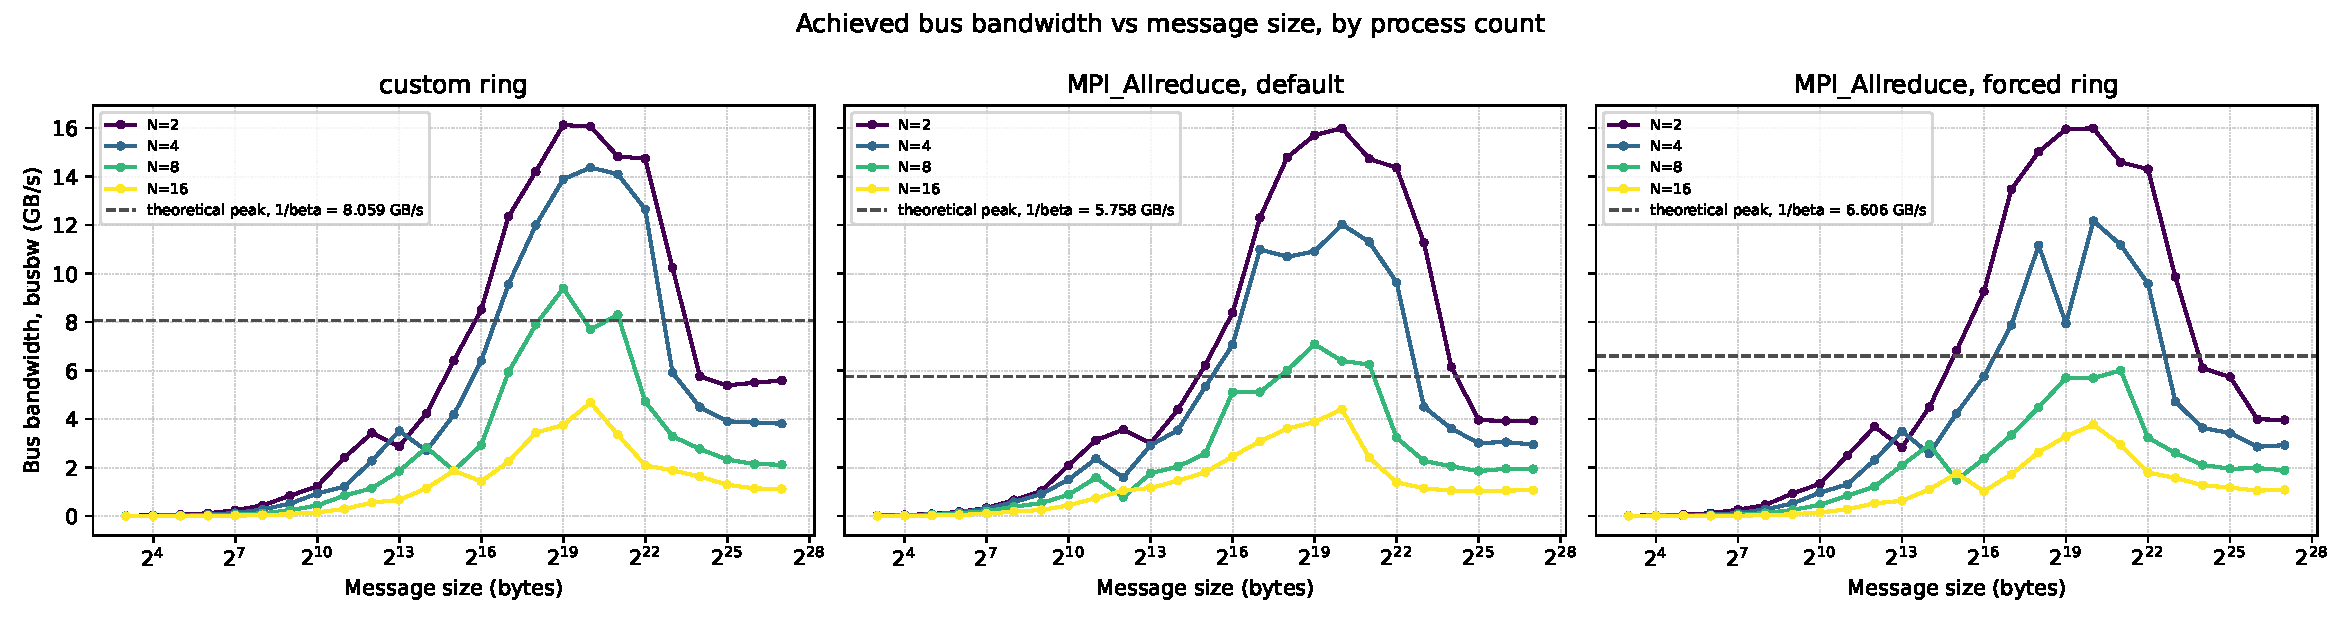
\includegraphics[width=\textwidth]{figures/busbw_vs_size.pdf}
\caption{Achieved bus bandwidth versus message size, log-scaled on the size axis, for $N \in \{2,4,8,16\}$, one panel per algorithm variant. The dashed line in each panel is that variant's fitted theoretical peak, $1/\beta$.}
\label{fig:busbw-vs-size}
\end{figure}

Table~\ref{tab:summary} quotes the two ends of the sweep at $N=16$, the most demanding process count. At 8~bytes every variant sits at a small fraction of a percent of its fitted peak, the latency-bound floor. At 128~MiB, the memory-bound far end, the custom ring reaches the highest absolute bus bandwidth of the three (1.120~GB/s, against 1.083 for the forced vendor ring and 1.070 for the default selection), though as a percentage of its own higher fitted asymptote that is a smaller fraction.

\begin{table}[htbp]
\centering
\begin{tabular}{lrrrr}
\toprule
Algorithm & busbw @ 8B (GB/s) & \% peak & busbw @ 128MiB (GB/s) & \% peak \\
\midrule
ring & 0.0013 & 0.02 & 1.120 & 13.90 \\
mpi-default & 0.0066 & 0.12 & 1.070 & 18.58 \\
mpi-ring & 0.0070 & 0.11 & 1.083 & 16.39 \\
\bottomrule
\end{tabular}

\caption{Achieved busbw and percent of that variant's fitted theoretical peak at the smallest (8~B) and largest (128~MiB) swept message sizes, at $N=16$: the most demanding process count in the sweep and therefore the most informative single configuration to summarize (averaging across $N$ would blend together regimes with very different busbw at the same message size and would not describe any one real configuration).}
\label{tab:summary}
\end{table}

\subsection{The head-to-head: two different comparisons}
\label{sec:head-to-head}

The central experimental result is not a single winner but the difference between two comparisons, which is exactly what benchmarking against both vendor variants (Section~\ref{sec:mca-forcing}) was designed to expose. Table~\ref{tab:headtohead} shows median times at $N=16$ across the size range.

\begin{table}[htbp]
\centering
\begin{tabular}{rrrr}
\toprule
Message size & custom ring ($\mu$s) & default ($\mu$s) & forced ring ($\mu$s) \\
\midrule
8~B      & 11.55     & 2.26      & 2.16 \\
64~B     & 11.08     & 2.41      & 11.97 \\
4~KiB    & 13.74     & 7.29      & 14.54 \\
64~KiB   & 85.72     & 49.86     & 119.21 \\
1~MiB    & 419.67    & 446.33    & 521.03 \\
16~MiB   & 19243.90  & 29920.40  & 24616.60 \\
128~MiB  & 224656.00 & 235199.00 & 232361.00 \\
\bottomrule
\end{tabular}
\caption{Median completion time at $N=16$ (lower is better). Against the \emph{default} selection the custom ring is roughly five times slower at 8~B and only overtakes it around 1~MiB. Against Open~MPI's \emph{own ring}, forced via MCA, the custom ring tracks it almost exactly from 64~B onward and beats it from 64~KiB up. The two rings behaving alike, while the default behaves entirely differently, is the step-count argument of Section~\ref{sec:step-count} measured directly.}
\label{tab:headtohead}
\end{table}

Against the default selection, the custom ring loses badly at small messages: 11.55~$\mu$s versus 2.26~$\mu$s at 8~bytes, a factor of roughly five, and it does not overtake the default until around 1~MiB. Against Open~MPI's own ring algorithm, the picture is completely different. From 64~bytes upward the forced vendor ring costs 11.97~$\mu$s at $N=16$ while the custom ring costs 11.08~$\mu$s: the two implementations of the same algorithm sit within about 8\% of each other, both roughly five times slower than the default selection. From 64~KiB upward the custom ring is the faster of the two rings, and by 16~MiB it completes in 19.2~ms against the vendor ring's 24.6~ms.

The one place the two rings diverge is at the very smallest sizes, 8~B and 32~B, where the forced vendor ring is as fast as the default selection rather than ring-like. The most likely explanation is that Open~MPI's tuned component retains a short-message special case that the MCA forcing does not fully override; the honest statement is that from 64~bytes upward, where the forcing demonstrably does take effect, the two rings behave like the same algorithm, because they are.

\subsection{Efficiency across the full sweep}

Figure~\ref{fig:efficiency-heatmap} extends this across every swept $(N, M)$ combination at once, with efficiency defined as achieved busbw over the fitted $1/\beta$ and the color scale allowed to run past 1 so the cache-resident band is not clipped away. The pattern is consistent across all three variants: efficiency is near zero across the small-message columns regardless of $N$, where the latency term of Equation~\ref{eq:hockney} dominates; it then rises through a bright band above the $1/\beta$ reference at the cache-resident middle sizes; and it falls back below 1 at the memory-bound largest sizes. The message size at which efficiency first lifts off the floor shifts right, toward larger messages, as $N$ grows, exactly as Equation~\ref{eq:hockney} predicts: the latency term scales with $N-1$, so more of the size axis stays latency-bound at larger $N$.

\begin{figure}[htbp]
\centering
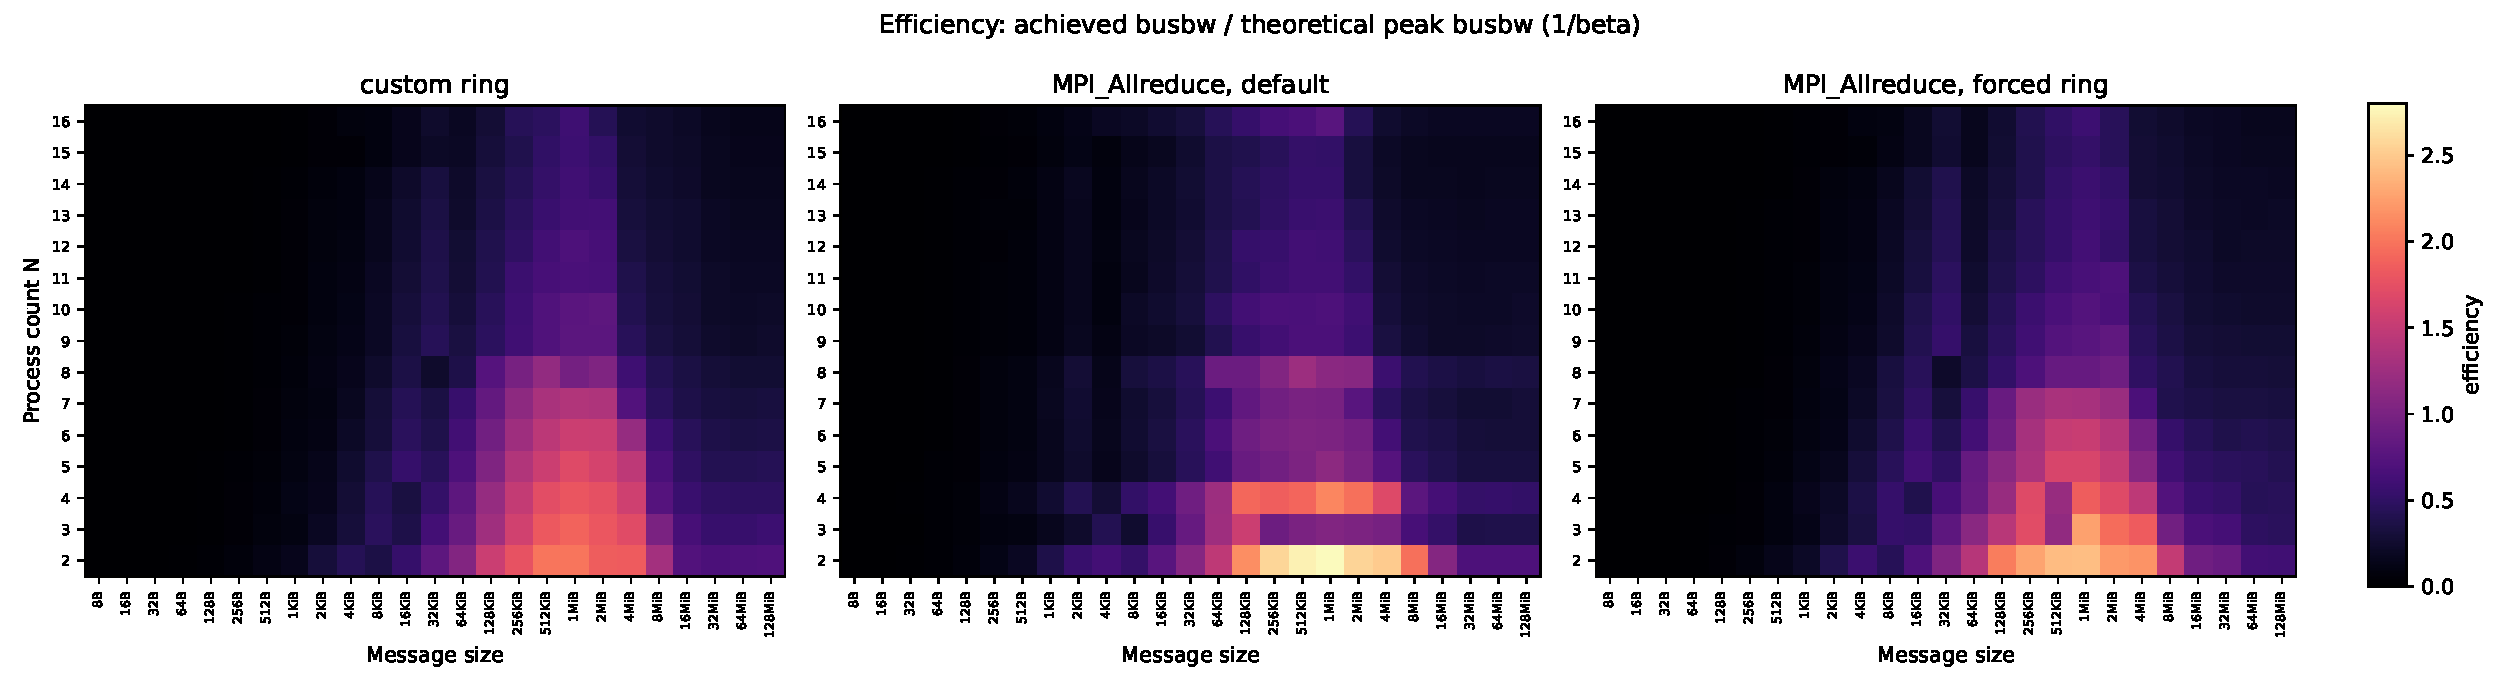
\includegraphics[width=\textwidth]{figures/efficiency_heatmap.pdf}
\caption{Efficiency (achieved busbw divided by that variant's fitted theoretical peak) across every swept process count and message size, one panel per algorithm variant. Values above 1 are the cache-resident sizes that beat the full-range sustained-bandwidth average, not a violation of the model.}
\label{fig:efficiency-heatmap}
\end{figure}

\subsection{Decomposing the latency floor}

Figure~\ref{fig:latency-decomposition} isolates the smallest swept message size and, for the custom ring specifically, breaks the cost model's prediction into its two additive terms per process count, alongside both the measured time and a raw \texttt{MPI\_Send}/\texttt{MPI\_Recv} ping-pong one-way latency taken on the same hardware in the same run (\texttt{apps/pingpong}, using the same one-way-latency-from-round-trip convention as OSU Micro-Benchmarks' \texttt{osu\_latency} \citep{osu2024benchmarks}).

Three things are visible at once. First, the bandwidth term is not merely small but numerically irrelevant: at 8~bytes it never exceeds $0.0019~\mu$s against a latency term of several microseconds, so at this size $T$ is the latency term and nothing else. Second, the raw ping-pong one-way latency is \textbf{0.1585~$\mu$s}, so a ring whose every step cost exactly one bare point-to-point message would take $2(N-1) \times 0.1585~\mu$s: that is the dashed "ideal floor" line, the best any ring could do on this hardware. Third, and most usefully, the measured time sits \emph{on} that floor for most of the range. Up to about $N=14$ the custom ring's measured 8-byte time tracks the ideal floor closely, meaning its per-step cost really is close to a bare point-to-point send and there is very little synchronization overhead to speak of.

The exception is the top of the range. At $N=15$ and $N=16$ the measured time jumps well above the floor, reaching 11.55~$\mu$s at $N=16$ against a floor of 4.7~$\mu$s. The shaded region in Figure~\ref{fig:latency-decomposition} is that excess, and it is the rank-synchronization overhead made visible: it is small and roughly flat while ranks are cheap to schedule, and it grows abruptly once they are not. A likely cause on this specific CPU is its hybrid topology (8 performance cores, each with two hardware threads, plus 12 efficiency cores): past a certain rank count the ring's slowest participant, which is what \texttt{MPI\_MAX} across ranks selects, starts landing on a hardware thread that shares execution resources with a sibling, or on a slower core, and every one of the $2(N-1)$ steps then waits on that straggler. Section~\ref{sec:discussion} takes up what this means and what it does not.

\begin{figure}[htbp]
\centering
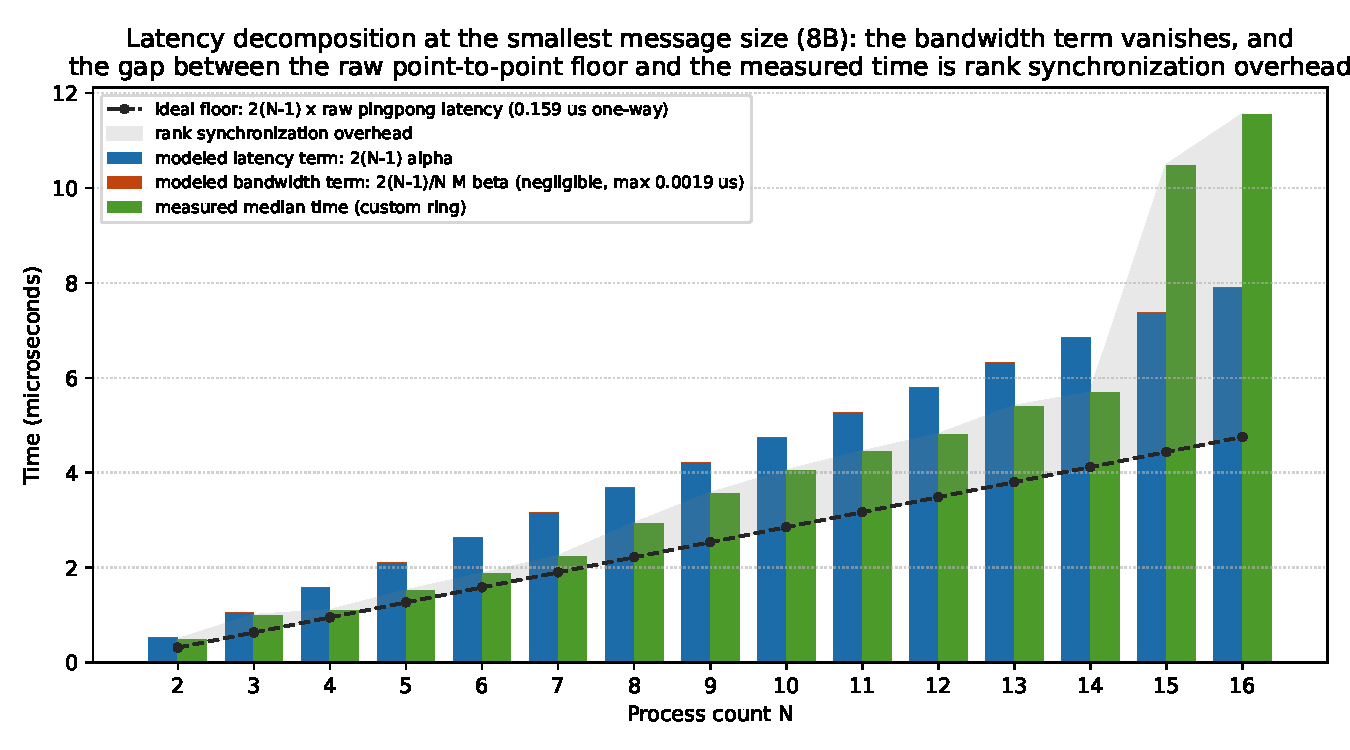
\includegraphics[width=\textwidth]{figures/latency_decomposition.pdf}
\caption{At the smallest swept message size (8~B), the ring's modeled latency term $2(N-1)\alpha$ and modeled bandwidth term $2\frac{N-1}{N}M\beta$ (the latter negligible, at most $0.0019~\mu$s), against the measured median time and against an ideal floor of $2(N-1)$ raw point-to-point latencies. The shaded gap between the floor and the measured time is rank synchronization overhead: near zero up to $N \approx 14$, then growing sharply.}
\label{fig:latency-decomposition}
\end{figure}

\section{Discussion}
\label{sec:discussion}

\subsection{Two distinct small-message bottlenecks}

Section~\ref{sec:results} shows the same latency-bound floor at small message sizes across every algorithm variant, and the cost model of Equation~\ref{eq:hockney} explains why in a way that separates two mechanisms which are easy to conflate into a single vague "small messages are slower."

\textbf{Pipeline fill latency} is structural. With only $N$ chunks and no further sub-chunking, every one of the $2(N-1)$ steps pays the full per-message latency $\alpha$ regardless of how small $M$ is; that fixed cost does not amortize over a smaller payload the way the bandwidth term does. As $M \to 0$, $\text{busbw} = M/T$ collapses toward zero simply because $T$ floors out at $2(N-1)\alpha$ while the numerator keeps shrinking. This is the flat region every panel of Figure~\ref{fig:busbw-vs-size} shows, and Figure~\ref{fig:latency-decomposition} confirms it directly: at the smallest swept size the modeled bandwidth term is negligible next to the modeled latency term at every $N$. The magnitude is concrete rather than abstract. With the custom ring's fitted $\alpha = 0.264~\mu$s, the predicted floor at $N=16$ is $2(16-1) \times 0.264 \approx 7.9~\mu$s, which is the right order for the 11.6~$\mu$s actually measured at 8 bytes, the remainder being the synchronization cost discussed next.

\textbf{Rank synchronization overhead} is a different, and non-structural, cost sitting on top of that floor. Step $s+1$ on rank $r$ cannot start until rank $r$'s own step $s$ has completed \emph{and} its neighbor has actually sent, so the operation runs at the speed of its slowest participant, which is exactly what the \texttt{MPI\_MAX} reduction of Section~\ref{sec:experimental-setup} measures. Stragglers and scheduling jitter therefore inflate the measured time on top of whatever the hardware's genuine point-to-point latency is. Figure~\ref{fig:latency-decomposition} is what makes this measurable rather than asserted, by putting the measured 8-byte time next to an ideal floor of $2(N-1)$ raw point-to-point latencies (0.1585~$\mu$s each, measured on the same hardware in the same run).

The answer is more interesting than a single constant. Averaged over the whole sweep, the fit puts the ring's per-step $\alpha$ at 0.264~$\mu$s against that 0.1585~$\mu$s bare latency, a gap of roughly 0.105~$\mu$s per step. But the per-$N$ view shows that average is hiding a threshold. Up to about $N=14$ the measured time sits essentially \emph{on} the ideal floor: the implementation's per-step cost really is close to a bare point-to-point send, and synchronization overhead is small. At $N=15$ and $N=16$ it departs sharply, reaching 11.55~$\mu$s against a 4.7~$\mu$s floor. So the honest statement is not "the ring pays a fixed 0.105~$\mu$s of synchronization per step" but "the ring pays almost no synchronization overhead until rank placement turns against it, and then it pays a great deal."

The most likely mechanism is this CPU's hybrid topology: 8 performance cores with two hardware threads each, plus 12 slower efficiency cores. Nothing is oversubscribed at $N=16$ on a 28-thread machine, so this is not classical core contention. It is that the \emph{slowest} rank sets the pace, and past a certain count some rank inevitably lands on a hyperthread sibling or an efficiency core and becomes a straggler that all $2(N-1)$ steps then wait on. This is worth flagging as a property of the measurement platform rather than of ring-allreduce: on a homogeneous cluster, or with explicit rank binding to performance cores only, the effect would be expected to weaken or disappear, and confirming that is a natural follow-up.

\subsection{Why a correct, bandwidth-optimal ring still loses at small messages}

Section~\ref{sec:step-count}'s step-count table is the other half of the story, and the three-variant comparison of Section~\ref{sec:head-to-head} turns it from an argument into a measurement.

Ring-allreduce is bandwidth-optimal, its total data movement is asymptotically independent of $N$, but it is not \emph{step}-optimal: it pays $2(N-1)$ sequential round trips where an algorithm built on recursive halving and doubling, such as the one Rabenseifner describes and \citet{thakur2005optimization} analyze, pays only $O(\log N)$. At $N=16$ that is 30 steps against 8, and every one of those extra steps costs at least one $\alpha$. Open~MPI's \texttt{coll/tuned} component exposes exactly those alternatives as separately selectable algorithms (Section~\ref{sec:mca-forcing} lists \texttt{recursive\_doubling} and \texttt{rabenseifner} in its enumerator), and its default selection is free to pick them for whatever size and process count it judges best.

The tempting but wrong conclusion from "my ring is five times slower than \texttt{MPI\_Allreduce} at 8 bytes" is that the implementation is poor. The forced-ring variant refutes that directly. When Open~MPI is made to run \emph{the same algorithm}, its own ring costs 11.97~$\mu$s at $N=16$ and 64~bytes, against this project's 11.08~$\mu$s: the two rings agree to within about 8\%, and both are roughly five times slower than the default selection. The gap to the default is therefore not an implementation gap at all. It is the price of the algorithm, paid identically by a mature vendor implementation and a from-scratch one, and it is precisely the $2(N-1)$ versus $O(\log N)$ step count that Table~\ref{tab:step-count} predicts. Benchmarking only against the default would have produced a number that looks like a verdict on code quality and is nothing of the sort.

Where the two rings do differ is instructive in the opposite direction. Table~\ref{tab:fits}'s fitted constants say the custom ring has the worse per-message latency ($\alpha = 0.264~\mu$s against the vendor ring's $0.113~\mu$s) but the better inverse bandwidth ($1/\beta = 8.06$~GB/s against 6.61~GB/s), and the head-to-head confirms it: the vendor ring wins the smallest sizes, the custom ring wins from 64~KiB upward, completing 16~MiB at $N=16$ in 19.2~ms against 24.6~ms. A plausible reading is that Open~MPI's ring is more careful about per-message setup while this implementation's straightforward, contiguous, non-blocking chunk exchange moves bulk bytes with less overhead per byte. That is a real and defensible outcome for a from-scratch implementation: competitive with, and at large messages faster than, the vendor's own ring, while paying more for each of its steps.

\subsection{Limitations}

Every measurement this report analyzes is single-node, gathered on the one workstation of Section~\ref{sec:experimental-setup} under Open~MPI's shared-memory transport. Two consequences follow and should be stated plainly. First, the cache-resident busbw peak, and the efficiency band that rises above 1 before falling back, are artifacts of shared memory: they would not appear over a real network fabric, where per-byte cost is set by the link rather than by whether the working set fits in L3. This is also why the linear cost model fits only loosely here ($R^2$ between 0.28 and 0.33), and a network-bound sweep would be expected to track it far better. Second, the fitted $\alpha$ folds in shared-memory handshake and scheduling costs that a network's own latency would replace rather than merely add to, so the 0.105~$\mu$s synchronization overhead quantified above is specific to this transport, even though the mechanism producing it is not.

A real multi-node sweep is therefore the single most valuable extension, and \texttt{scripts/run\_slurm\_sweep.sbatch} exists so this project's methodology extends to that setting without modification. Nothing about the algorithm, the cost model, or the analysis pipeline is single-node-specific; only the dataset gathered so far is.

The comparison is also CPU-only. GPU-to-GPU collectives, NCCL's actual production setting, add device-to-host transfer costs, NVLink or PCIe topology, and GPUDirect-style optimizations that a CPU MPI benchmark cannot speak to; that comparison is out of scope here and left to Section~\ref{sec:conclusion}'s future work rather than attempted with a mismatched proxy.

\subsection{What a segmented ring would change}

The pipeline fill latency mechanism above suggests a concrete next optimization, not attempted in this implementation: sub-chunking each of the $N$ pieces further and pipelining transmission of those sub-chunks across steps, so that a step's communication for one sub-chunk can overlap with communication for another instead of every step waiting on one full-size round trip. That directly attacks the $2(N-1)\alpha$ term, which this report's own data identifies as the ring's actual handicap: it is what makes the ring lose to the default selection at small messages, and it is the fixed cost a lower-step algorithm avoids. The bandwidth term is where this ring already wins, beating even the vendor's own ring above 64~KiB, so latency, not byte-moving, is the part still worth optimizing. That Open~MPI ships a \texttt{segmented\_ring} algorithm as a separate enumerator value (Section~\ref{sec:mca-forcing}) is a strong hint that this is the standard next move, and Section~\ref{sec:conclusion} lists it as the highest-value follow-up specifically because this report's data, not intuition, is what points at it.

\section{Conclusion}
\label{sec:conclusion}

This project implemented ring-allreduce from scratch directly on MPI point-to-point primitives, with the two-phase reduce-scatter and all-gather structure, its edge cases, and its bandwidth-optimal data volume all treated as first-class requirements rather than details to fill in later, and validated against both vendor \texttt{MPI\_Allreduce} and an independently-computed reference across a test matrix that deliberately includes non-power-of-two process counts and the zero-size-chunk cases a smaller test matrix would miss. The analysis pipeline fits this project's own hardware constants, $\alpha$ and $\beta$, from measured data via a weighted least-squares procedure whose necessity (and whose alternative's failure mode) was itself demonstrated empirically rather than assumed, and uses those constants to separate pipeline fill latency from rank synchronization overhead as two distinct, individually quantified small-message bottlenecks, and to explain, via step count rather than vague appeal to "vendor optimization," the specific circumstances under which this implementation can lose to a vendor \texttt{MPI\_Allreduce}'s own algorithm selection despite being bandwidth-optimal. On the single-node Microsoft MPI measurements analyzed here, that loss is real below a few kilobytes and reverses above it, the ring becoming the faster of the two by up to a factor of two through the cache-resident message sizes, which is the expected consequence of a bandwidth-optimal but step-heavy algorithm rather than a defect.

The limitations, stated plainly rather than buried, are those of a single-node run. The transport underneath is Microsoft MPI's shared memory, not a network fabric, which is what produces the cache-resident bus-bandwidth peak and the modest fit of the linear cost model (Section~\ref{sec:dataset-note}); and Microsoft MPI's lack of \texttt{coll/tuned} controls means the forced ring-versus-ring comparison, which would isolate implementation quality from algorithm choice, was not among the variants that could be measured. Both are addressed by the same step, an Open~MPI multi-node sweep via \texttt{scripts/run\_slurm\_sweep.sbatch}, regenerating this report from that output (\texttt{make report} against the new CSVs) without changing a single line of the methodology described here.

Beyond that, three extensions would most directly build on this project's own findings rather than add unrelated scope. First, and most directly motivated by Section~\ref{sec:discussion}'s own data: a segmented, pipelined ring that overlaps communication across steps, attacking the latency term this report's decomposition specifically identified as the one still worth optimizing. Second, a naive gather-to-one-rank-then-broadcast baseline, purely as a third comparison point that would make concrete, in this project's own numbers, exactly why a from-scratch ring was worth building in the first place. Third, a real multi-node sweep via \texttt{scripts/run\_slurm\_sweep.sbatch}, extending every method in this report to a setting where network fabric, rather than shared memory, sets the real $\alpha$ and $\beta$. A GPU and NCCL comparison is deliberately not on this list: it is a different hardware regime with its own transfer costs and topology effects that a CPU MPI benchmark cannot speak to responsibly, and is noted here only as future work rather than attempted with a mismatched proxy.


\bibliographystyle{plainnat}
\bibliography{references}

\end{document}
